\documentclass{article}
\usepackage[utf8]{inputenc}
\usepackage[hidelinks]{hyperref}
\usepackage[spanish]{babel}
\usepackage[left=2cm,right=2cm,top=2cm,bottom=2cm]{geometry}
\usepackage{graphicx}
\usepackage{pdflscape}
\usepackage{listings}

\lstset {
    frame = single,
    breaklines = true
}


\begin{document}

\begin{titlepage}

\title{\textbf{
    {\Huge Práctica 4: Digitalizar una cinta magnética de ZX Spectrum}\\
    {\Large Sistemas Legados}
}}
\author{
    Pedro Allué Tamargo (758267)
    \and
    Juan José Tambo Tambo (755742)
    \and
    Jesús Villacampa Sagaste (755739)
}
\date{\today}
\clearpage\maketitle
\thispagestyle{empty}
\tableofcontents
\end{titlepage}

\section{Introducción}

En esta práctica se va a proceder a digitalizar una cinta que contiene programas para el \textit{ZX Spectrum\footnote{\url{https://es.wikipedia.org/wiki/Sinclair_ZX_Spectrum}}}. La cinta proporcionada por el profesor parecía estar en perfecto estado.\\

El procedimiento a seguir consiste en obtener un archivo \textit{Wav} a partir del contenido de la cinta de \textit{cassette} que posteriormente será convertido a formato \textit{.tzx}. Finalmente, se comprobará si la digitalización ha sido correcta utilizando un emulador \textit{ZX Spectrum}.\\

Para obtener el archivo \textit{WAV}, se utilizará \textit{Audacity}, un editor de audio de código abierto multiplataforma que permite grabar contenido de un \textit{cassette} y modificar el archivo de audio obtenido cortando elementos sobrantes y aplicando efectos que mejoren la calidad.\\
Para la conversión de archivos \textit{WAV} a \textit{TZX} se utilizará la herramienta \textit{MakeTZX\footnote{\url{http://ramsoft.bbk.org.omegahg.com/maketzx.html}}}. Esta herramienta se puede utilizar mediante línea de comandos o utilizando una interfaz gráfica que simplifica el trabajo del usuario.\\
Finalmente, para comprobar que se ha realizado la digitalización correctamente, se utilizará el emulador \textit{ZX Spectrum} \textit{FUSE}\footnote{\url{http://fuse-emulator.sourceforge.net/}}.


\section{Esfuerzos invertidos}

\begin{itemize}
    \item Pedro Allué Tamargo: Búsqueda de información de grabación de cintas, transformación a \textit{tzx} y mejora de los ficheros \textit{wav} obtenidos.
        \begin{itemize}
            \item Tiempo invertido: 5 horas
        \end{itemize}
    \item Juan José Tambo Tambo: Obtención de archivos \textit{WAV}, edición de los mismos, transformación en \textit{tzx}, uso de herramienta \textit{TAPIR}.
        \begin{itemize}
            \item Tiempo invertido: 20 horas
        \end{itemize}
    \item Jesús Villacampa Sagaste: Grabación de cintas en formato \textit{wav}, transformación a \textit{tzx} y pruebas con \textit{Fuse}
        \begin{itemize}
            \item Tiempo invertido: 10 horas
        \end{itemize}
\end{itemize}


\section{Proceso de digitalización}


Para digitalizar las cintas se han seguido los pasos indicados en el enunciado de la práctica. El proceso de digitalización se compone de varios pasos. Para la realización de esta parte nos hemos apoyado en el siguiente \href{https://ezcontents.org/zx-spectrum-tape-conversion}{tutorial}.\\

El primer paso se corresponde con la grabación de la cinta utilizando \textit{Audacity}. Para ello, se debe conectar el \textit{cassette} a la entrada de audio del ordenador mediante un cable minijack macho - minijack macho. Seguidamente, desde \textit{Audacity}, se deben configurar los parámetros de grabación para evitar que el audio esté muy saturado o demasiado bajo. Para ello se selecciona la entrada de audio deseada, se presiona en \textit{``comenzar monitorización''} y se reproduce la cinta, regulando el volumen de salida intentando que los picos de máxima intensidad se mantengan en -3db.
\begin{figure}[h!]
    \centering
    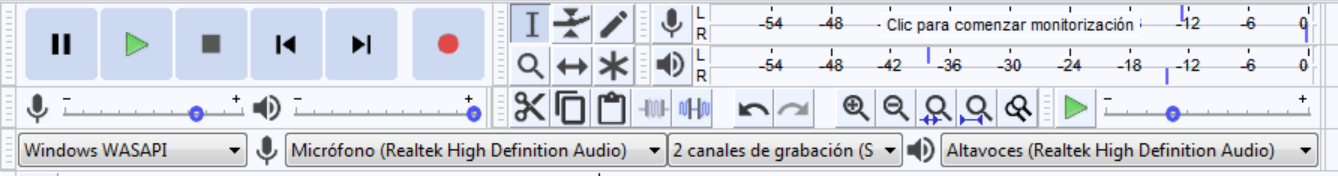
\includegraphics[scale=0.5]{images/configuracion-audacity.PNG}
    \caption{Configuración de grabación desde \textit{Audacity}}
    \label{fig:conf-audacity}
\end{figure}

En la primera grabación, se configuró la grabación en \textit{stereo}. Al terminar la grabación de la primera cara de la cinta (cara A), se recorta el audio sobrante para evitar fallos, es decir, el trozo de pista desde que se comienza a grabar hasta que comienza a reproducir el contenido.\\
\begin{figure}[h!]
    \centering
    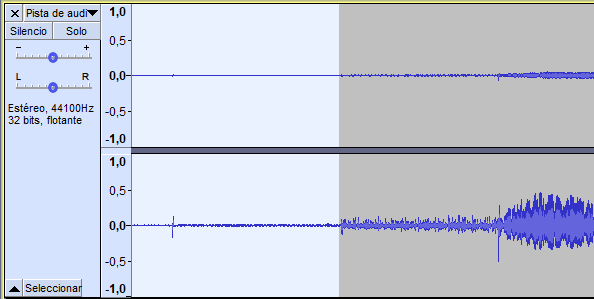
\includegraphics[scale=0.5]{images/audio-sobrante.png}
    \caption{Eliminación de audio sobrante de la grabación}
    \label{fig:audio-sobrante}
\end{figure}

Una vez se ha grabado el contenido de la cinta, se exporta el en formato \textit{WAV} codificación \texttt{Unsigned 8-bit PCM} (\texttt{Archivo/Exportar/Exportar como WAV}). Seguidamente, desde la interfaz gráfica de \textit{MakeZTX} se debe seleccionar el archivo \textit{WAV} a convertir desde \texttt{File to convert} y se selecciona en \texttt{Start}. Esta herramienta muestra una salida que indica qué bloques se han podido recuperar de la cinta y si ha habido error o no en ese bloque. El resultado obtenido por esta herramienta al aplicar la conversión en la primera grabación realizada se puede observar en la Figura \ref{fig:stereo-bad}\\

\begin{figure}[h!]
    \centering
    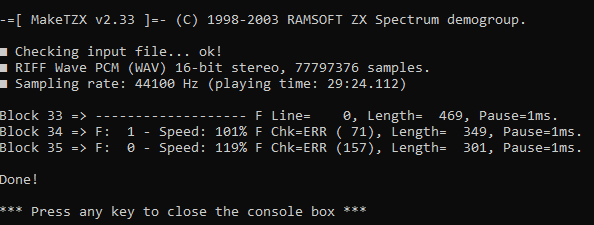
\includegraphics[scale=0.5]{images/stereo-bad.png}
    \caption{Salida del programa \textit{MakeTZX} tras convertir la primera grabación}
    \label{fig:stereo-bad}
\end{figure}

Al intentar cargar el archivo \textit{TZX} generado por \textit{MakeTZX} en \textit{FUSE}, no se obtuvo ningún resultado. \\

En un segundo intento, se ha probado a convertir el archivo grabado en formato \textit{stereo} a \textit{mono}. Para ello, desde el proyecto de \textit{Audacity} procedemos a eliminar el canal de audio que no ha recibido ninguna entrada seleccionando en \texttt{Dividir pista estéreo a mono} y eliminando el canal sin entrada. \\
Si se repite el procedimiento comentado anteriormente para obtener el \textit{TZX}, se puede observar que ha reconocido correctamente dos programas (\textit{Airwolf} y \textit{SCUBA}) y otro programa que no se ha leido correctamente (bloque 19).\\

\begin{figure}[h!]
    \centering
    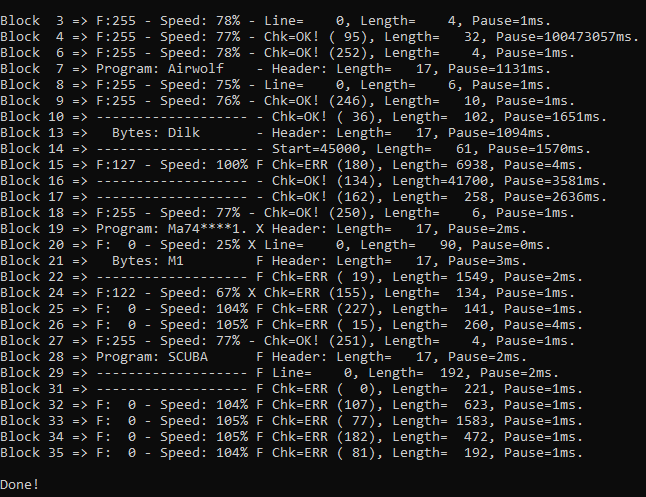
\includegraphics[scale=0.4]{images/stereo-to-mono.png}
    \caption{Salida del programa \textit{MakeTZX} tras convertir la grabación de \textit{stereo} a \textit{mono}}
    \label{fig:stereo-to-mono}
\end{figure}

Además, siguiendo el manual de la herramienta \textit{MakeTZX}\footnote{\url{http://ramsoft.bbk.org.omegahg.com/mtzxman.html}} se sabe que todos los bloques que contienen el símbolo `-' tras el nombre del bloque, han sido decodificados correctamente; Los seguidos por `F' indican que el bloque está corrupto, por lo que no se ha podido recuperar correctamente y los seguidos por `X' indican que el \textit{checksum} es incorrecto pero no se detectan errores.\\

Si emulamos el nuevo archivo \textit{TZX} con \textit{FUSE}, siguiendo las indicaciones presentadas en el enunciado de la práctica, se debe cargar el primer programa, por lo que se debe escribir \texttt{LOAD ``''}. La combinación de teclas necesarias para ejecutar este comando es: \texttt{j + (ctrl + p) + (ctrl + p)}. Sin embargo, aunque la salida de \textit{MakeTZX} indicara que se habían obtenidos algunos programas, desde \textit{FUSE} no se pudo acceder a ninguno, mostrándose únicamente \textit{Bytes: Dilk}(Figura ).\\
\begin{figure}[h!]
    \centering
    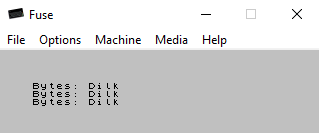
\includegraphics[scale=0.6]{images/fuse-stereo-to-mono.png}
    \caption{Emulación en \textit{FUSE} incorrecta}
    \label{fig:fuse-stereo-to-mono}
\end{figure}

Tras observar varios tutoriales y leer el manual del programa \textit{MakeTZX}, se observó que se podían aplicar distintos \textit{loader} desde la interfaz gráfica del programa. Hasta ahora, no se había aplicado ninguno (configuración por defecto). De esta manera, se probó a convertir el archivo \textit{WAV} utilizando las distintas opciones de \textit{loaders} que proporciona el programa, obteniendo el mejor resultado con la opción \textit{Normal (ROM)}. Si se ejecuta el \textit{TZX} obtenido con, se puede observar que se ha podido digitalizar correctamente el programa \textit{Airwolf} de la cinta y se puede interactuar con él. Para poder cargar el programa, desde el emulador \textit{FUSE}, se ha cargado el archivo \textit{TZX}, se ha hecho \textit{reset} del emulador y se ha cargado el programa con el comando \texttt{LOAD ``Airwolf''}. La salida de la conversión desde \textit{MakeTZX} ha indicado que ha podido leer otros programas como \textit{sabre wulf, GIFT-GODS, SCUBA y MONTY MOLE}, aunque fallaba al intentar cargar el programa. El único caso especial es el del programa \textit{MONTY MOLE} el cual, al intentar cargar, aparecía el siguiente error: \texttt{R Tape loading error, 0:1}\\

\begin{figure}[h!]
    \centering
    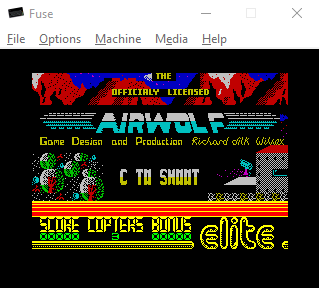
\includegraphics[scale=0.6]{images/airwolf.png}
    \caption{Emulación correcta del programa \textit{Airwolf}}
    \label{fig:airwolf}
\end{figure}

Se realizaron algunas grabaciones más de la cara A de la cinta y, al no obtener mejora, se decidió utilizar otro reproductor de cintas. Este reproductor permitía elegir el tipo de reproducción de la cinta (\textit{stereo o  mono}). En un nuevo intento, se seleccionó el modo \textit{mono} desde el reproductor y desde \textit{Audacity}, obteniendo así un solo canal de grabación. Tras exportar el archivo \textit{wav} y convertirlo a \textit{tzx}, se observó que el número de bloques decodificados por la herramienta \textit{MakeTZX} eran mayores que los obtenidos hasta el momento. Al probar el archivo obtenido en \textit{FUSE}, se observó que, además del programa ``Airwolf'' anterior, se podría jugar sin problema al programa ``Gift-Gods'' y ``Scuba Dive'' (Figura \ref{Fig:giftGods} y \ref{Fig:scuba}). Además, cargando todos los programas de la cinta se observó que aún aparecían algunos más que no se ejecutaban correctamente.\\

\begin{figure}[!htb]
   \begin{minipage}{0.48\textwidth}
     \centering
     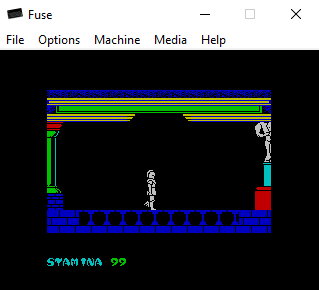
\includegraphics[width=.7\linewidth]{images/gift-gods.png}
     \caption{Juego \textit{Gift-Gods}}\label{Fig:giftGods}
   \end{minipage}\hfill
   \begin{minipage}{0.48\textwidth}
     \centering
     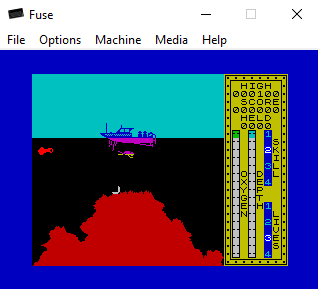
\includegraphics[width=.7\linewidth]{images/scuba.png}
     \caption{Juego \textit{Scuba Dive} }\label{Fig:scuba}
   \end{minipage}
\end{figure}

A partir de esta grabación que proporcionó buenos resultados, se intentó mejorar la calidad de la grabación para obtener más programas. Para ello, desde \textit{Audacity}\footnote{Se han seguido las recomendaciones encontradas en \url{https://andalinux.wordpress.com/2018/08/23/audacity-convertir-vinilos-o-cintas-a-formato-digital-y-exportar-el-resultado-en-temas-individuales-de-manera-automatica/}} se pueden aplicar los efectos de \texttt{Normalizar, reducción de ruido y amplificar}. Con el primero los evitamos los picos de ruido "normalizando" la grabación a los decibelios deseados (en nuestro caso se selecciona -3 db); El segundo efecto, como su nombre indica permite reducir la cantidad de ruido presente en la grabación, sobre todo en las partes entre dos programas en las que solo se escucha el ruido de la cinta; El último, permite amplificar el sonido de la grabación en caso de que se haya grabado demasiado bajo (se recomienda dejar los parámetros por defecto). 
Aplicando los efectos anteriores, se han obtenido algunos programas más, aunque en distintos archivos \textit{tzx} ya que unas configuraciones favorecían a la correcta decodificación de algunos programas y con otros efectos se obtenían otros programas. \par
Además de los efectos mencionados de \textit{Audacity}, desde la herramienta \textit{MakeTZX} se puede seleccionar la opción \textit{digital filter} la cual permite la reducción de ruido de la grabación, mejorando la calidad del archivo decodificado (los parámetros se han dejado por defecto). Esta opción se recomienda utilizar si se obtiene el error \texttt{R Tape loading error, 0:1} al ejecutar en el emulador.

Tras realizar varias pruebas con las diferentes posibles configuraciones mencionadas anteriormente, se ha observado que los mejores resultados se obtienen tras aplicar el efecto de \texttt{Reducción de ruido} y normalizar. Además, al contrario de lo que se pensaba en pruebas anteriores, desde \textit{MakeTZX}, el tipo de decodificación que produce mejores resultados es \textit{None}, ante \textit{Normal (ROM)}.\\

Al final, se han obtenido dos juegos más a parte de los mencionados con anterioridad: ``PSSST'' y ``Atic Atac'' (Figuras \ref{Fig:pst} y \ref{Fig:AticAtac}). Además, se obtiene otro programa, ``Lerm Tape Copier 6'' (Figura \ref{fig:advertencia}), el cual se encarga de hacer copias de los programas de la cinta y cargarlos a velocidad normal\footnote{\url{https://www.mutant-caterpillar.co.uk/shop/product_info.php?products_id=4127}}.\\

\begin{figure}[!htb]
   \begin{minipage}{0.32\textwidth}
     \centering
     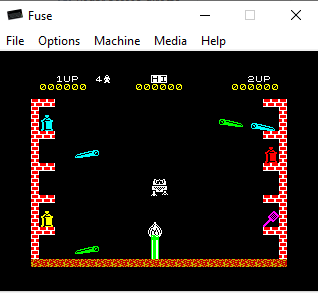
\includegraphics[width=\linewidth]{images/pst.png}
     \caption{Juego \textit{PSST}}\label{Fig:pst}
   \end{minipage}\hfill
   \begin{minipage}{0.32\textwidth}
     \centering
     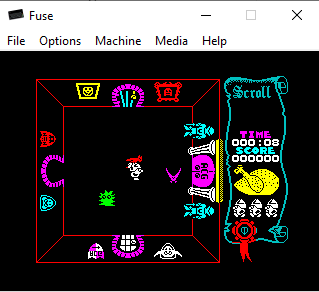
\includegraphics[width=\linewidth]{images/atic-atac.png}
     \caption{Juego \textit{Atic Atac} }\label{Fig:AticAtac}
   \end{minipage}
   \minipage{0.32\textwidth}%
  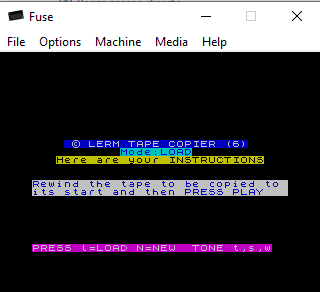
\includegraphics[width=\linewidth]{images/advertencia.png}
  \caption{Programa LTC6}\label{fig:advertencia}
\endminipage
\end{figure}

Observando la salida de la herramienta \textit{MakeTZX} e intentando cargar todo el contenido de la cinta, se ha observado que existen más programas que no se han podido digitalizar correctamente. Estos programas son ``ManicMiner'', ``sabre wulf'' y ``Monty Mole''. En el caso de los dos primeros, al intentar cargar daba error: \texttt{R Tape loading error}, con códigos de error distintos. En el caso de ``Monty Mole'', la pantalla se volvía de color rosa hasta que finalmente aparecía el mismo error que en los anteriores. Se han realizado algunas grabaciones más intentando modificar algunos parámetros como el volumen de entrada de la grabación o cambiando la frecuencia de grabación a 48000Hz (\texttt{Audacity/Editar/Preferencias/Calidad/Frecuencia de muestreo}) pero sin conseguir ninguna mejora notable.\\

Por último, como algunos programas no se encuentran en el mismo \textit{tzx}\footnote{Esto se debe a que se han usado distintas configuraciones para obtener los programas}, se ha hecho uso de la herramienta \textit{TAPIR}. Con ella, se permite obtener bloques de un archivo \textit{tzx} y copiarlos en otro. De esta manera, se han seleccionado los bloques correspondientes a determinados programas y se han juntado en un solo archivo (Figura \ref{fig:tapir}). 

\begin{figure}[h!]
    \centering
    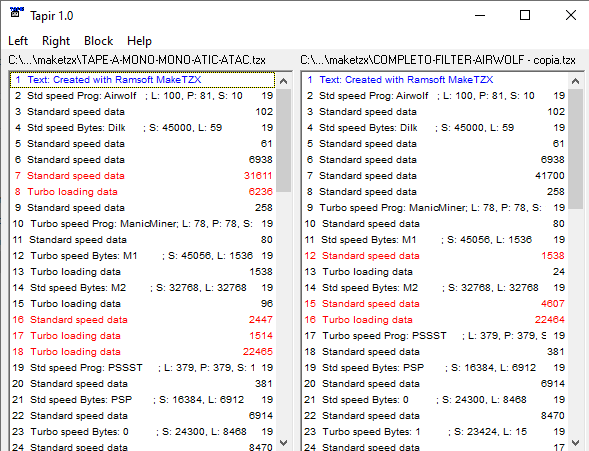
\includegraphics[scale=0.6]{images/tapir.png}
    \caption{Uso de la herramienta \textit{TAPIR}}
    \label{fig:tapir}
\end{figure}

El caso del programa ``Monty Mole'' mencionado con anterioridad es especial ya que es el último almacenado en la cinta. Tras grabar el contenido de la \textbf{cara b} de la cinta, se observó que los primeros bloques de esta hacían referencia a \textit{monty} por lo que se consideró la posibilidad de que añadiendo los primeros bloques de la \textbf{cara b} al final del \textit{tzx} de la \textbf{cara a} se podría obtener el programa. Usando la herramienta \textit{TAPIR} y juntando bloques de amabas caras se obtuvo el programa completo ``Monty Mole'' (Figura \ref{fig:montyMole}). Los programas ``sabre wulf'' y ``Manic Miner'' no se han podido obtener ya que hay un par de bloques que están corruptos a la hora de la decodificación. Se ha intentado obtener esos bloques aplicando distintas configuraciones y filtros pero continuaban dando error durante la decodificación.\\

\begin{figure}[h!]
    \centering
    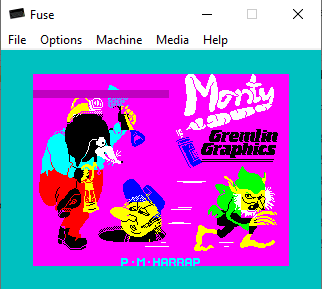
\includegraphics[scale=0.6]{images/monty-mole.png}
    \caption{Programa ``Monty Mole'' obtenido desde las dos caras de la cinta}
    \label{fig:montyMole}
\end{figure}

\newpage
Para la \textbf{cara B} de la cinta se han seguido los procedimientos comentados anteriormente. La obtención de los programas fue un proceso menos tedioso que en la \textbf{cara A} porque es de menor duración y ya se tenían ciertos conocimientos acerca de cómo realizar la grabación y las modificaciones necesarias sobre el audio para obtener la mejor calidad posible.

Finalmente, con la ayuda de la herramienta \textit{TAPIR} para obtener bloques correctos entre distintos archivos \textit{tzx}, se han conseguido obtener 3 programas de la \textbf{cara B} de a cinta: ``Deathchase'', ``Herbie'' y ``Fairlight'' (Figuras \ref{Fig:deathchase}, \ref{Fig:Herbie} y \ref{fig:fairlight}). El único problema encontrado en esta cinta es que el último juego (\textit{Fairlight}) no se consiguió obtener correctamente, ya que el final de la cinta produce demasiado ruido y no se ha podido conseguir ninguna mejora para obtener la información.\\

\begin{figure}[!htb]
   \begin{minipage}{0.32\textwidth}
     \centering
     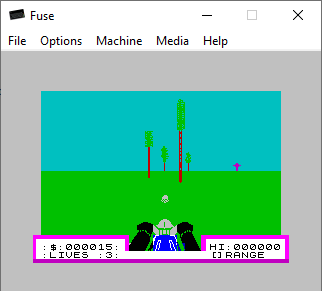
\includegraphics[width=\linewidth]{images/deathchase.png}
     \caption{Juego \textit{Deathchase}}\label{Fig:deathchase}
   \end{minipage}\hfill
   \begin{minipage}{0.32\textwidth}
     \centering
     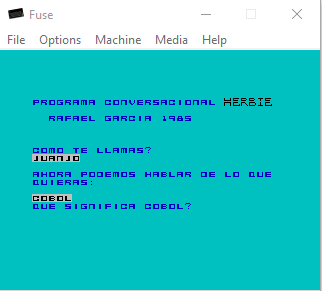
\includegraphics[width=\linewidth]{images/herbie.png}
     \caption{Programa conversacional \textit{Herbie} }\label{Fig:Herbie}
   \end{minipage}
   \minipage{0.32\textwidth}%
  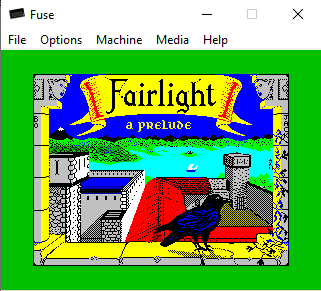
\includegraphics[width=\linewidth]{images/fairlight.png}
  \caption{Programa \textit{Fairlight}}\label{fig:fairlight}
\endminipage
\end{figure}

\subsection{Problemas encontrados} 
La mayoría de problemas aparecieron al comienzo de la realización de la práctica, ya que las primeras grabaciones poseían mucho ruido y no se obtenía ningún dato en limpio. Además, el problema principal se encontraba en el reproductor de cintas ya que no era de buena calidad. Sólo se notificó de este problema una vez se había probado con otro reproductor (el usado finalmente) ya que éste sí que obtenía buenos resultados. \\

Hasta que no se encontró la herramienta \textit{TAPIR}, la digitalización resultó un proceso mucho más complicado ya que se tenía que conseguir la digitalización correcta de un programa entero en vez de juntar los bloques correctos de distintos \textit{tzx} con configuraciones distintas.


\section{Conclusiones}

La realización de la práctica ha sido un proceso interesante, consiguiendo un buen resultado finalmente a diferencia de las expectativas que se tenían al principio. \\

Si no hubiera sido por el cambio de reproductor de cintas, no se habría podido realizar la práctica.\\

La digitalización es un proceso tedioso que, si no se tiene experiencia previa, puede generar muchos problemas. Una vez se poseen las herramientas necesarias, termina siendo un proceso entretenido y más simple.

\end{document}
